\begin{thmBox}[Lemma]{26.1}[lem:26.1]
    Let \( Y \) be a subspace of \( X \).
    Then \( Y \) is compact if and only if every covering of \( Y \) by sets
    open in \( X \) contains a finite subcollection covering \( Y \).

    \baseRule

    \begin{proofBox}
        Suppose that \( Y \) is compact and \( \mathcal{A} = 
        \{ A_{ i } \}_{ i \in I } \) is an open covering of \( Y \) by sets 
        open in \( X \).
        We want to show that there exists a finite subcollection in 
        \( \mathcal{A} \) that covers \( Y \).

        \baseSkip

       We start off by using the fact that \( \mathcal{A} \) is an open covering
       of \( Y \) by sets open in \( X \); by definition of what a covering 
       is for a subspace, we have that 
        \begin{equation*}
            Y \subset \bigcup_{ i \in I } A_{ i }
        \end{equation*}
        Which is equivalent to saying that 
        \begin{equation*}
            Y
            =
            Y \cap \left( \bigcup_{ i \in I } A_{ i } \right)
            =
            \bigcup_{ i \in I } ( A_{ i } \cap Y )
        \end{equation*}
        Thus, we see that the collection \( \mathcal{A}' = 
        \{ A_{ i } \cap Y \mid i \in I \} \) is an open covering of \( Y \) 
        by sets open in \( Y \).

        \baseSkip

        Since \( Y \) is compact, we see that it has a finite subcollection
        in \( \mathcal{A}' \), say 
        \begin{equation*}
            \{ A_{ i_{ 1 } } \cap Y , \ldots , A_{ i_{ n } } \cap Y \}
        \end{equation*}
        that covers \( Y \); that is, 
        \begin{equation*}
            \bigcup_{ j = 1 }^{ n } ( A_{ i_{ j } } \cap Y )
            =
            Y
        \end{equation*}
        Notice that 
        \begin{equation*}
            Y
            =
            \bigcup_{ j = 1 }^{ n } ( A_{ i_{ j } } \cap Y )
            =
            Y \cap \left( \bigcup_{ j = 1 }^{ n } A_{ i_{ j } } \right)
        \end{equation*}
        which tells us that 
        \begin{equation*}
            Y \subset \bigcup_{ j = 1 }^{ n } A_{ i_{ j } }
        \end{equation*}
        Thus, we end up getting that \( \{ A_{ i_{ 1 } } , \ldots , 
        A_{ i_{ n } } \} \) is a finite subcollection of \( \mathcal{A} \) that 
        covers \( Y \).

        \baseSkip

        Conversely, suppose that every covering of \( Y \) by sets open in 
        \( X \) contains a finite subcollection covering \( Y \); we wish to 
        prove that \( Y \) is compact.

        \baseSkip

        Let \( \mathcal{A}' = \{ A_{ i }' \}_{ i \in I } \) be any open 
        covering of \( Y \) by sets open in \( Y \).
        Our goal is to show that there exists a finite subcollection of 
        \( \mathcal{A}' \) that covers \( Y \).
        For each \( i \), we can choose a set \( A_{ i } \) open in \( X \)
        such that 
        \begin{equation*}
            A_{ i }'
            =
            A_{ i } \cap Y
        \end{equation*}
        by definition of \( A_{ i }' \) being open in \( Y \) under the subspace
        topology.
        We can see that the collection \( \mathcal{A} = 
        \{ A_{ i } \}_{ i \in I } \) is a covering of \( Y \) by sets open in 
        \( X \):
        \begin{equation*}
            Y 
            = 
            \bigcup_{ i \in I } A_{ i }'
            =
            \bigcup_{ i \in I } ( A_{ i } \cap Y )
            =
            Y \cap \bigcup_{ i \in I } A_{ i }
            \implies 
            Y \subset \bigcup_{ i \in I } A_{ i }
        \end{equation*}
        By our hypothesis, we have that there exists some finite subcollection
        of \( \mathcal{A} \), say \( \{ A_{ i_{ 1 } } , \ldots , 
        A_{ i_{ n } } \} \), such that it covers \( Y \).
        Thus, we have by definition of a covering for a subspace that
        \begin{equation*}
            Y
            \subset
            \bigcup_{ j = 1 }^{ n } A_{ i_{ j } }
        \end{equation*}
        Notice that 
        \begin{equation*}
            Y
            =
            Y \cap \left( \bigcup_{ j = 1 }^{ n } A_{ i_{ j } } \right)
            =
            \bigcup_{ j = 1 }^{ n } ( Y \cap A_{ i_{ j } } )
            =
            \bigcup_{ j = 1 }^{ n } A_{ i_{ j } }'
        \end{equation*}
        From this, we get that \( \{ A_{ i_{ 1 } }' , \ldots , 
        A_{ i_{ n } }' \} \) is a subcollection of \( \mathcal{A}' \) that
        covers \( Y \).
    \end{proofBox}
\end{thmBox}

\begin{thmBox}{Variation of [\hyperlink{lem:26.1}{Lemma 26.1}]}[thm:26.1]
    Let \( X \) be a topological space and \( Y \) a subspace of \( X \).
    Let \( A \) be a subset such that \( A \subset Y \subset X \).
    \( A \) is compact in \( X \) if and only if \( A \) is compact in \( Y \).

    \baseRule

    \begin{proofBox}
        Let's say that \( A \) is compact in \( X \).
        By [\hyperlink{lem:26.1}{Lemma 26.1}], we have that every covering of \( A \)
        by sets open in \( X \) contains a finite subcollection covering \( A \).
        We want to show that \( A \) is compact in \( Y \), meaning that for every 
        covering of \( A \) by sets open in \( Y \), there exists a finite subcollection
        covering \( A \).
        
        \baseSkip

        Let \( \mathcal{U} \) be an open covering of \( A \) by sets open in \( Y \).
        By definition of what a covering is for a subspace, we see that 
        \begin{equation*}
            A \subset \bigcup_{ U \in \mathcal{U} } U
        \end{equation*}
        By definition of the subspace topology, we see that for each 
        \( U \in \mathcal{U} \), there exists some open set \( V \) of \( X \) such that
        \( U = V \cap Y \).
        Let us denote the collection of all such open sets \( V \) of \( X \) as 
        \( \mathcal{V} \).
        We can see that 
        \begin{equation*}
            A \subset \bigcup_{ U \in \mathcal{U} } U
            \iff 
            A \subset \bigcup_{ V \in \mathcal{V} } ( V \cap Y )
            \iff 
            A \subset \left( \bigcup_{ V \in \mathcal{V} } V \right) \cap Y
            \implies 
            A \subset \bigcup_{ V \in \mathcal{V} } V
        \end{equation*}
        which tells us that \( \mathcal{V} \) is an open covering of \( A \) by sets 
        open in \( X \).

        \baseSkip

        Since \( A \) is compact in \( X \), we see that there exists some finite
        subcollection \( \{ V_{ 1 } , \ldots , V_{ n } \} \) of \( \mathcal{V} \) such
        that it covers \( A \).
        Hence, it follows that 
        \begin{equation*}
            A \subset \bigcup_{ i = 1 }^{ n } V_{ i }
            \text{ and }
            A \subset Y
            \implies 
            A \subset \left( \bigcup_{ i = 1 }^{ n } V_{ i } \right) \cap Y
            \iff 
            A \subset \bigcup_{ i = 1 }^{ n } ( V_{ i } \cap Y )
            \iff 
            A \subset \bigcup_{ i = 1 }^{ n } U_{ i }  
        \end{equation*}
        which tells us that \( \{ U_{ 1 } , \ldots , U_{ n } \} \) is a finite 
        subcollection of \( \mathcal{U} \) such that it openly covers \( A \) in 
        \( Y \).
        Since our choice of open cover \( \mathcal{U} \) in \( Y \) was arbitrary,
        we have that \( A \) must be compact in \( Y \).

        \baseSkip

        Let's now say that \( A \) is compact in \( Y \).
        We want to show that \( A \) is compact in \( X \), meaning that for every 
        covering of \( A \) by sets open in \( X \), there exists a finite subcollection
        covering \( A \).
        
        \baseSkip

        Let \( \mathcal{U} \) be an open covering of \( A \) by sets open in \( X \).
        By definition of what a covering is for a subspace, we see that 
        \begin{equation*}
            A \subset \bigcup_{ U \in \mathcal{U} } U
        \end{equation*}
        Since \( A \subset Y \) as well, we see that
        \begin{equation*}
            A \subset \left( \bigcup_{ U \in \mathcal{U} } U \right) \cap Y
            \iff 
            A \subset \bigcup_{ U \in \mathcal{U} } ( U \cap Y )
        \end{equation*}
        Under the subspace topology, we have that \( U \cap Y \) is open in \( Y \) for
        each \( U \in \mathcal{U} \).
        Thus, we have that \( \{ U \cap Y \mid U \in \mathcal{U} \} \) is an open 
        covering of \( A \) by sets open in \( Y \).
        
        \baseSkip

        Since \( A \) is compact in \( Y \), we see that there exists a finite 
        subcollection \( \{ U_{ 1 } \cap Y , \ldots , U_{ n } \cap Y \} \) such that 
        it covers \( A \).
        Hence it follows that 
        \begin{equation*}
            A \subset \bigcup_{ i = 1 }^{ n } ( U_{ i } \cap Y )
            \iff 
            A \subset \left( \bigcup_{ i = 1 }^{ n } U_{ i } \right) \cap Y
            \implies 
            A \subset \bigcup_{ i = 1 }^{ n } U_{ i } 
        \end{equation*}
        which tells us that \( \{ U_{ 1 } , \ldots , U_{ n } \} \) is a finite 
        subcollection of \( \mathcal{U} \) such that it covers \( A \).
        Since our choice of open cover \( \mathcal{U} \) in \( X \) was arbitrary,
        we have that \( A \) must be compact in \( X \).
    \end{proofBox}
\end{thmBox}

\begin{thmBox}{26.2}[thm:26.2]
    Every closed subspace of a compact space is compact.

    \baseRule

    \begin{proofBox}
        Let \( X \) be compact and \( A \subset X \) be closed.
        Let \( \mathcal{U} = \{ U_{ i } \}_{ i \in I } \) be an open cover of 
        \( A \).
        We want to show that \( \mathcal{U} \) admits a finite subcover of 
        \( A \).

        \baseSkip

        To do so, we note that \( \mathcal{U} \cup \{ X \setminus A \} \) is an 
        open cover of \( X \).
        Since \( X \) is compact, it follows that such an open cover admits a 
        finite subcover of \( X \).
        If this subcover contains the set \( X \setminus A \), then we can 
        discard \( X \setminus A \); otherwise, we can leave the subcover alone.
        The resulting subcover is a finite subcover of \( \mathcal{U} \) that
        covers \( A \).
    \end{proofBox}
\end{thmBox}

\begin{thmBox}{26.3}[thm:26.3]
    Every compact subspace of a Hausdorff space is closed.

    \baseRule

    \begin{proofBox}
        Let \( Y \) be a compact subspace of the Hausdorff space \( X \).
        We shall prove that \( X \setminus Y \) is open, so that \( Y \) is
        closed.

        \baseSkip

        Let \( x_{ 0 } \) be a point of \( X \setminus Y \).
        We show that there is a neighborhood of \( x_{ 0 } \) that is 
        disjoint from \( Y \).
        For each point \( y \in Y \), we are always able to choose disjoint
        neighborhoods \( U_{ y } \) and \( V_{ y } \) of the points 
        \( x_{ 0 } \) and \( y \), respectively (using the Hausdorff condition).
        We can see by construction that
        the collection \( \{ V_{ y } \mid y \in Y \} \) is a covering of \( Y \)
        by the sets open in \( X \); since \( Y \) is compact, we see that 
        there are finitely many of them \( V_{ y_{ 1 } } , \ldots , 
        V_{ y_{ n } } \) that cover \( Y \).

        \baseSkip

        Let us now consider the following two sets:
        \begin{equation*}
            V 
            =
            V_{ y_{ 1 } } \cup \ldots \cup V_{ y_{ n } }
            \quad \mathrm{and} \quad 
            U = U_{ y_{ 1 } } \cap \ldots \cap U_{ y_{ n } }
        \end{equation*}
        We can see clearly that both \( U \) and \( V \) are open; namely,
        we see that compactness of \( Y \) is what allowed for us to 
        obtain a \textit{finite} intersection of the corresponding 
        neighborhoods \( U_{ y_{ j } } \) of \( x_{ 0 } \).  
        We can see as well that \( V \)
        contains \( Y \), and it is disjoint from the open set \( U \);
        for if \( z \) is a point of \( V \), then \( z \in V_{ y_{ i } } \) for
        some \( i \).
        Hence \( z \notin U_{ y_{ i } } \), and so \( z \notin U \).

        \begin{figure}[H]
            \centering
            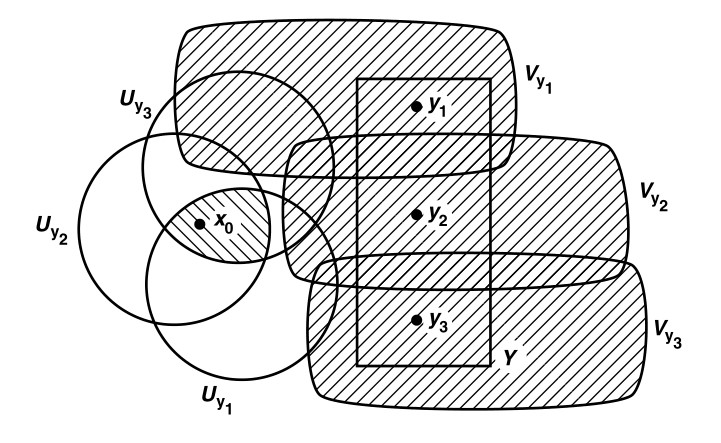
\includegraphics[ width = 0.5\linewidth ]{figures/Section 26/thm_26-1.jpg}
            \caption{A visual on the disjointness of \( U \)}
            \label{fig:26.1}
        \end{figure}

        As a result, we see that \( U \) is a neighborhood of \( x_{ 0 } \) 
        disjoint from \( Y \), as desired.
        Thus, we see that \( Y \) is closed in \( X \).
    \end{proofBox}
\end{thmBox}

\begin{thmBox}[Lemma]{26.4}[lem:26.4]
    If \( Y \) is a compact subspace of the Hausdorff space \( X \) and 
    \( x_{ 0 } \) is not in \( Y \), then there exist disjoint open sets
    \( U \) and \( V \) of \( X \) containing \( x_{ 0 } \) and \( Y \),
    respectively.

    \baseRule

    \begin{proofBox}
        This result is proved while proving 
        [\hyperlink{thm:26.3}{Theorem 26.3}].
    \end{proofBox}
\end{thmBox}

\begin{thmBox}{Extending Lemma 26.4}[thm:26.4]
    Let \( X \) be Hausdorff. 
    Let \( K \) and \( L \) be disjoint compact subsets of \( X \).
    Then there exists disjoint open neighborhoods \( U \) of \( K \)
    and \( V \) of \( L \).

    \baseRule

    \begin{proofBox}
        For all \( x \in K \), we have that there exists disjoint open 
        neighborhoods \( U_{ x } \) of \( x \) and \( V_{ x } \subset L \)
        (this follows from [\hyperlink{lem:26.4}{Lemma 26.4}]).
        \( \{ U_{ x } \}_{ x \in K } \) is an open cover of \( K \).
        Since \( K \) is compact, we see that it admits a finite subcover:
        \( \{ U_{ x_{ 1 } } , \ldots ,  U_{ x_{ n } } \} \).

        \baseSkip

        Define 
        \begin{equation*}
            U
            =
            \bigcup_{ i = 1 }^{ n } U_{ x_{ i } }
            \quad \mathrm{and} \quad 
            V
            =
            \bigcap_{ i = 1 }^{ n } V_{ x_{ i } }
        \end{equation*}
        We can see that \( U \) is an open neighborhood of \( K \) and \( V \)
        is an open neighborhood of \( L \) since any \( V_{ x } \) contains 
        \( L \).
        We have that \( U \cap V = \emptyset \), which results in \( K \) and
        \( L \) to be disjoint. 
    \end{proofBox}
\end{thmBox}

\begin{thmBox}{26.5}[thm:26.5]
    The image of a compact space under a continuous map is compact.

    \baseRule

    \begin{proofBox}
        Let \( f: X \rightarrow Y \) be a continuous function and \( X \) is 
        compact.
        We want to show that \( f ( X ) \) is compact.

        \baseSkip

        Let's say that we are given some open cover of \( f ( X ) \), say 
        \( \mathcal{A} = \{ A_{ i } \}_{ i \in I } \).
        Our goal is to show that \( \mathcal{A} \) admits a finite subcover of 
        \( f ( X ) \).

        \baseSkip

        Then we see that \( \{ f^{ -1 } ( A_{ i } ) \}_{ i \in I } \) are an 
        open cover of \( X \).
        Now since \( X \) is compact, we see that there exists a finite subcover
        of \( X \), say \( \{ f^{ -1 } ( A_{ i_{ 1 } } ) , \ldots , f^{ -1 } ( A_{ i_{ n } } ) \} \).
        From here, we see that \( \{ A_{ i_{ 1 } } , \ldots , A_{ i_{ n } } \} \) is an open cover of \( f ( X ) \).

        \begin{equation*}
            f ( X ) \subset \bigcup_{ i \in I } A_{ i }
            \iff 
            X \subset f^{ -1 } \left( \bigcup_{ i \in I } A_{ i } \right)
            \iff
            X
            \subset
            \bigcup_{ i \in I } f^{ -1 } ( A_{ i } ) 
        \end{equation*}
    \end{proofBox}
\end{thmBox}

\begin{thmBox}{26.6}[thm:26.6]
    Let \( f: X \rightarrow Y \) be a bijective continuous function.
    If the domain \( X \) is compact and the codomain \( Y \) is Hausdorff, 
    then \( f \) is a homeomorphism.

    \baseRule

    \begin{proofBox}
        All we need to do is to show that \( f^{ -1 } \) is continuous so that
        \( f \) is a homeomorphism.
        To do so, it suffices to show that \( f \) is a closed map -- that is,
        images of closed sets are closed.
        Doing so will results in \( f^{ -1 } \) to be continuous.

        \baseSkip

        If \( A \) is closed in \( X \), then \( A \) must be compact by 
        [\hyperlink{thm:26.2}{Theorem 26.2}]. 
        Therefore, we have by [\hyperlink{thm:26.5}{Theorem 26.5}] that 
        \( f ( A ) \) is compact in \( Y \).
        Now since \( Y \) is Hausdorff, it follows that \( f ( A ) \) is 
        closed in \( Y \) by [\hyperlink{thm:26.3}{Theorem 26.3}], which results
        in \( f \) to be a closed map.

        \baseSkip

        We will now go about showing that \( f^{ -1 }: Y \rightarrow X \),
        which is defined since \( f \) is bijective, is continuous.
        We shall do so by showing that \( ( f^{ -1 } )^{ -1 } ( A ) \) is 
        closed in \( Y \) whenever \( A \) is closed in \( X \).
        Now since \( f \) is bijective, we get
        \begin{equation*}
            ( f^{ -1 } )^{ -1 } ( A )
            =
            f ( A )
        \end{equation*}
        is closed in \( Y \) because \( f \) is a closed map
    \end{proofBox}
\end{thmBox}

\begin{thmBox}{26.7}[thm:26.7]
    The product of finitely many compact spaces is compact.

    \baseRule

    \begin{proofBox}
        It suffices to show that the result holds for a product of two compact
        sets; the case for the product of finitely many compact spaces follows
        immediately from induction.
        
        \baseSkip

        Let \( X \) and \( Y \) be compact spaces.
        Let \( \mathcal{A} \) be an open covering of \( X \times Y \).
        Our goal is to show that there exists a finite subcollection of 
        \( \mathcal{A} \) such that it openly covers \( X \times Y \).

        \baseSkip

        Given \( y \in Y \), it follows that the space \( X \times \{ y \} \)
        is homeomorphic to the space \( X \) (using the same map as in 
        [\hyperlink{lem:26.8}{Lemma 26.8}]).
        Since \( X \) was compact, it follows that the slice 
        \( X \times \{ y \} \) is compact, which allows for us 
        to find a finite subcollection \( A_{ 1 } , \ldots , A_{ n } \) of 
        \( \mathcal{A} \) such that it openly covers \( X \times \{ y \} \).
        As a result, we see that 
        \begin{equation*}
            N
            =
            A_{ 1 } \cup \ldots \cup A_{ n }
        \end{equation*}
        is an open set containing \( X \times \{ y \} \).

        \baseSkip

        By [\hyperlink{lem:26.8}{Lemma 26.8}], it follows that \( N \)
        contains a tube \( X \times V \) about \( X \times \{ y \} \),
        where \( V \) is open in \( Y \).
        It must then be the case that \( X \times V \) is covered by finitely 
        many elements \( A_{ 1 } , \ldots , A_{ n } \) of \( \mathcal{A} \).
        As a result, we have that for each \( b \in Y \), we can choose a 
        neighborhood \( V_{ b } \) of \( b \) such that the tube 
        \( X \times V_{ b } \) can be covered by finitely many elements of
        \( \mathcal{A} \).
        The collection of all the neighborhoods \( V_{ b } \) is an open
        covering of \( Y \); therefore by compactness of \( Y \), there 
        exists a finite subcollection
        \begin{equation*}
            \{ V_{ 1 } , \ldots , V_{ k } \}
        \end{equation*}
        that openly covers \( Y \).
        The union of the tubes 
        \begin{equation*}
            X \times V_{ 1 } , \ldots , X \times V_{ k }
        \end{equation*}
        is all of \( X \times Y \), and since each may be covered by finitely 
        many elements of \( \mathcal{A} \), it follows that \( X \times Y \)
        can also be covered by finitely many elements of \( \mathcal{A} \).
        
        \baseSkip

        Thus, we see that \( X \times Y \) is compact.
    \end{proofBox}
\end{thmBox}

\begin{thmBox}[Lemma]{Homeomorphic Spaces to Slices}[lem:26.8.1]
    Let \( X \) and \( Y \) be topological spaces.
    WLOG, consider the slice \( X \times \{ y \} \).
    We have that \( X \times \{ y \} \) is homeomorphic to \( X \).

    \baseRule

    \begin{proofBox}
        Let us consider the following map:
        \begin{equation*}
            f: X \rightarrow X \times \{ y \}
            \quad \mathrm{where} \quad 
            f ( x ) = x \times y 
            \quad \forall x \in X
        \end{equation*}
        We can see that this map is clearly bijective.
        Hence, we know that there exists an inverse of \( f \) given as follows:
        \begin{equation*}
            f^{ -1 }: X \times \{ y \} \rightarrow X
            \quad \mathrm{where} \quad 
            f^{ -1 } ( x \times y ) = x
            \quad \forall x \in X
        \end{equation*}
        We can see that \( f^{ -1 } \) is clearly continuous since it is
        the projection onto \( X \), which we already know is a continuous map.
        To show that \( f \) is continuous, let us consider any basic open set 
        \( U \times \{ y \} \) in \( X \times \{ y \} \), where \( U \) is an
        open set of \( X \).
        It follows that \( f^{ -1 } ( U \times \{ y \} ) = U \), which we know 
        is open.
        Thus, we have that \( f \) is continuous.

        \baseSkip

        Putting everything together results in us getting that \( f \) is 
        indeed a homeomorphism, which further results in \( X \times \{ y \} \)
        being homeomorphic to \( X \).
    \end{proofBox}
\end{thmBox}

\begin{thmBox}[Lemma]{26.8 (The Tube Lemma)}[lem:26.8]
    Consider the product space \( X \times Y \), where \( X \) is compact.
    If \( N \) is an open set of \( X \times Y \) containing the slice 
    \( X \times \{ y \} \) of \( X \times Y \), then \( N \) contains some 
    tube \( X \times V \) about \( X \times \{ y \} \), where \( V \) is a 
    neighborhood of \( y \) in \( Y \).

    \baseSkip

    In other words, there is a neighborhood \( V \) of \( y \) in \( Y \)
    such that \( N \) contains the entire set \( X \times V \).

    \baseRule

    \begin{proofBox}
        Let \( X \) be compact and \( y \in Y \) be given.
        Let \( N \) be an open neighborhood of \( X \times \{ y \} \) be given.
        Our goal is to show that there is a neighborhood \( V \) of \( y \) in
        \( Y \) such that \( N \) contains the entire set \( X \times V \).

        \baseSkip 

        Let us first start by covering \( X \times \{ y \} \) by basis elements 
        \( U \times W \) (for the topology of \( X \times Y \)) lying in 
        \( N \).
        By the [\hyperlink{lem:26.8.1}{lemma}] above, we see that 
        \( X \times \{ y \} \) is homeomorphic to \( X \).
        Thus, we have that \( X \) being compact implies that 
        \( X \times \{ y \} \) must be compact as well.
        Therefore, we can cover \( X \times \{ y \} \) by finitely many such
        basis elements:
        \begin{equation*}
            U_{ 1 } \times W_{ 1 }
            , \ldots , 
            U_{ n } \times W_{ n }
        \end{equation*}
        This is where we note that we assume that each basis element
        \( U_{ i } \times W_{ i } \) actually intersects 
        \( X \times \{ y \} \), since
        otherwise that basis element would be superfluous; we could discard it 
        from the finite collection and still have a covering of 
        \( X \times \{ y \} \).

        \baseSkip

        We now define 
        \begin{equation*}
            V 
            =
            W_{ 1 } \cap \ldots \cap W_{ n }
        \end{equation*}
        The set \( V \) is open, and it contains \( y \) because each set
        \( U_{ i } \times W_{ i } \) intersects \( X \times \{ y \} \).
        We claim that the sets \( U_{ i } \times W_{ i } \), which were
        chosen to cover the slice \( X \times \{ y \} \), actually cover
        the tube \( X \times V \) -- that is, we want to show that 
        \begin{equation*}
            X \times V \subset \bigcup_{ i = 1 }^{ n } 
            ( U_{ i } \times W_{ i } )
        \end{equation*}

        \baseSkip

        To verify this claim, we want to show that for any point
        \( a \times b \in X \times V \), we have that 
        \( a \times b \in U_{ i } \times W_{ i } \) for some \( i \).
        Let \( a \times b \) be a point of \( X \times V \).
        Consider the point \( a \times y \) of the slice \( X \times \{ y \} \)
        having the same \( x \)-coordinate as this point.
        Since \( \{ U_{ i } \times W_{ i } \}_{ i \in I } \) is a finite 
        open cover of \( X \times \{ y \} \), we have that \( a \times y \) 
        belongs to \( U_{ i } \times W_{ i } \) for some \( i \), so that 
        \( a \in U_{ i } \).
        However, since \( b \in V \), we see that \( b \in W_{ j } \) for 
        \textit{every} \( j \).
        Thus, it follows that \( a \times b \in U_{ i } \times W_{ i } \),
        which results in \( \{ U_{ i } \times W_{ i } \}_{ i \in I } \) to be 
        an open cover of \( X \times V \).

        \begin{figure}[H]
            \centering
            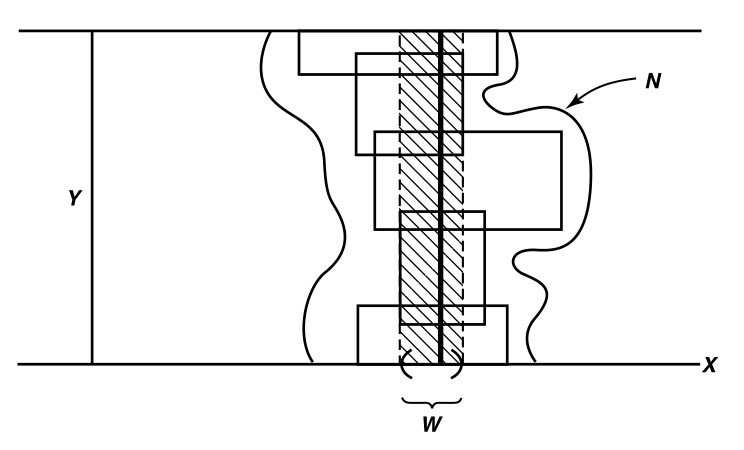
\includegraphics[ width = 0.5\linewidth ]{figures/Section 26/lem_26-8.jpg}
            \caption{A visual of the Tube Lemma}
            \label{fig:26-2}
        \end{figure}
    \end{proofBox}
\end{thmBox}

\begin{thmBox}{26.9}[thm:26.9]
    Let \( X \) be a topological space.
    Then \( X \) is compact if and only if every collection \( \mathcal{C} \) of
    closed sets in \( X \) having the finite intersection property, the 
    intersection \( \bigcap_{ C \in \mathcal{C} } C \) of all the elements of 
    \( \mathcal{C} \) is nonempty.

    \baseRule

    \begin{proofBox}
        Given a collection \( \mathcal{A} \) of subsets of \( X \), let
        \begin{equation*}
            \mathcal{C}
            =
            \{ X \setminus A \mid A \in \mathcal{A} \} 
        \end{equation*}
        be the collection of their complements.
        Then the following statements hold:
        \begin{enumerate}
            \item \( \mathcal{A} \) is a collection of open sets if and only if
                \( \mathcal{C} \) is a collection of closed sets.
            \item The collection \( \mathcal{A} \) covers \( X \) if and only if
                the intersection \( \bigcap_{ C \in \mathcal{C} } C \) of all 
                the elements of \( \mathcal{C} \) is empty.
            \item The finite subcollection 
            \( \{ A_{ 1 } , \ldots , A_{ n } \} \) of \( \mathcal{A} \) covers
            \( X \) if and only if the intersection of the corresponding 
            elements \( C_{ i } = X \setminus A_{ i } \) of \( \mathcal{C} \)
            is empty.
        \end{enumerate}
        The first statement follows immediately by definition of open and closed
        sets.
        The second and third follow from DeMorgan's law:
        \begin{equation*}
            X \setminus \left( \bigcup_{ i \in I } A_{ i } \right)
            =
            \bigcap_{ i \in I } ( X \setminus A_{ i } )
        \end{equation*}
        where some collection of \( \{ A_{ i } \}_{ i \in I } \) covers \( X \)
        if \( X \setminus \left( \bigcup_{ i \in I } A_{ i } \right) 
        = \emptyset \).
        From here, the proof will proceed in two steps: take the contrapositive
        of the theorem, and then the complement of the sets.

        \baseSkip

        The state that \( X \) is compact is equivalent to saying: "Given any
        collection \( \mathcal{A} \) of open subsets of \( X \), if
        \( \mathcal{A} \) covers \( X \), then some finite subcollection of 
        \( \mathcal{A} \) covers \( X \)."
        This statement is equivalent to the contrapositive, which is the 
        following: "Given any collection \( \mathcal{A} \) of open subsets of 
        \( X \), if no finite subcollection of \( \mathcal{A} \) covers \( X \),
        then \( \mathcal{A} \) does not cover \( X \)."

        \baseSkip

        Letting \( \mathcal{C} \) be, as earlier, the collection 
        \( \{ X \setminus A \mid A \in \mathcal{A} \} \) and applying 
        \( ( 1 ) - ( 3 ) \), we see that this statement is in turn equivalent
        to the following: "Given any collection \( \mathcal{C} \) of closed
        sets of \( X \), if every finite intersection of elements of 
        \( \mathcal{C} \) is nonempty, then the intersection of all the
        elements of \( \mathcal{C} \) is nonempty." This is just the condition
        of our theorem.
    \end{proofBox}
\end{thmBox}

\begin{thmBox}{Heine-Borel}[thm:26_heine-borel]
    A subset of \( \mathbb{R}^{ n } \) with the standard topology is compact in
    \( \mathbb{R}^{ n } \) if and only if it is both closed and \textbf{bounded}
    (which means that there is a finite upper limit to how far apart points in that subspace can be).

    \baseRule

    \begin{proofBox}

    \end{proofBox}
\end{thmBox} 